%%%%%%%%%%%%%%%%%%%%%%%%%%%%%%%%%%%%%%%%%
% Proceedings of the National Academy of Sciences (PNAS)
% LaTeX Template
% Version 1.0 (19/5/13)
%
% This template has been downloaded from:
% http://www.LaTeXTemplates.com
%
% Original author:
% The PNAStwo class was created and is owned by PNAS:
% http://www.pnas.org/site/authors/LaTex.xhtml
% This template has been modified from the blank PNAS template to include
% examples of how to insert content and drastically change commenting. The
% structural integrity is maintained as in the original blank template.
%
% Original header:
%% PNAStmpl.tex
%% Template file to use for PNAS articles prepared in LaTeX
%% Version: Apr 14, 2008
%
%%%%%%%%%%%%%%%%%%%%%%%%%%%%%%%%%%%%%%%%%

%----------------------------------------------------------------------------------------
%	PACKAGES AND OTHER DOCUMENT CONFIGURATIONS
%----------------------------------------------------------------------------------------

%------------------------------------------------
% BASIC CLASS FILE
%------------------------------------------------

%% PNAStwo for two column articles is called by default.
%% Uncomment PNASone for single column articles. One column class
%% and style files are available upon request from pnas@nas.edu.

%\documentclass{pnasone}
\documentclass{pnastwo}

%------------------------------------------------
% POSITION OF TEXT
%------------------------------------------------

%% Changing position of text on physical page:
%% Since not all printers position
%% the printed page in the same place on the physical page,
%% you can change the position yourself here, if you need to:

% \advance\voffset -.5in % Minus dimension will raise the printed page on the 
                         %  physical page; positive dimension will lower it.

%% You may set the dimension to the size that you need.

%------------------------------------------------
% GRAPHICS STYLE FILE
%------------------------------------------------

%% Requires graphics style file (graphicx.sty), used for inserting
%% .eps/image files into LaTeX articles.
%% Note that inclusion of .eps files is for your reference only;
%% when submitting to PNAS please submit figures separately.

%% Type into the square brackets the name of the driver program 
%% that you are using. If you don't know, try dvips, which is the
%% most common PC driver, or textures for the Mac. These are the options:

% [dvips], [xdvi], [dvipdf], [dvipdfm], [dvipdfmx], [pdftex], [dvipsone],
% [dviwindo], [emtex], [dviwin], [pctexps], [pctexwin], [pctexhp], [pctex32],
% [truetex], [tcidvi], [vtex], [oztex], [textures], [xetex]

\usepackage{float}
\usepackage{graphicx}
\usepackage{caption}
\graphicspath{{../figures/}}
%------------------------------------------------
% OPTIONAL POSTSCRIPT FONT FILES
%------------------------------------------------

%% PostScript font files: You may need to edit the PNASoneF.sty
%% or PNAStwoF.sty file to make the font names match those on your system. 
%% Alternatively, you can leave the font style file commands commented out
%% and typeset your article using the default Computer Modern 
%% fonts (recommended). If accepted, your article will be typeset
%% at PNAS using PostScript fonts.

% Choose PNASoneF for one column; PNAStwoF for two column:
%\usepackage{PNASoneF}
%\usepackage{PNAStwoF}

%------------------------------------------------
% ADDITIONAL OPTIONAL STYLE FILES
%------------------------------------------------

%% The AMS math files are commonly used to gain access to useful features
%% like extended math fonts and math commands.

\usepackage{amssymb,amsfonts,amsmath}
\usepackage{color}

%------------------------------------------------
% OPTIONAL MACRO FILES
%------------------------------------------------

%% Insert self-defined macros here.
%% \newcommand definitions are recommended; \def definitions are supported

%\newcommand{\mfrac}[2]{\frac{\displaystyle #1}{\displaystyle #2}}
%\def\s{\sigma}

%------------------------------------------------
% DO NOT EDIT THIS SECTION
%------------------------------------------------

%% For PNAS Only:
\contributor{Submitted to Proceedings of the National Academy of Sciences of the United States of America}
\url{www.pnas.org/cgi/doi/10.1073/pnas.0709640104}
\copyrightyear{2008}
\issuedate{Issue Date}
\volume{Volume}
\issuenumber{Issue Number}

%----------------------------------------------------------------------------------------

\begin{document}

%----------------------------------------------------------------------------------------
%	TITLE AND AUTHORS
%----------------------------------------------------------------------------------------

\title{Is essentiality of genes conserved in Enterobacteriaceae?} % For titles, only capitalize the first letter

%------------------------------------------------

%% Enter authors via the \author command.  
%% Use \affil to define affiliations.
%% (Leave no spaces between author name and \affil command)

%% Note that the \thanks{} command has been disabled in favor of
%% a generic, reserved space for PNAS publication footnotes.

%% \author{<author name>
%% \affil{<number>}{<Institution>}} One number for each institution.
%% The same number should be used for authors that
%% are affiliated with the same institution, after the first time
%% only the number is needed, ie, \affil{number}{text}, \affil{number}{}
%% Then, before last author ...
%% \and
%% \author{<author name>
%% \affil{<number>}{}}

%% For example, assuming Garcia and Sonnery are both affiliated with
%% Universidad de Murcia:
%% \author{Roberta Graff\affil{1}{University of Cambridge, Cambridge,
%% United Kingdom},
%% Javier de Ruiz Garcia\affil{2}{Universidad de Murcia, Bioquimica y Biologia
%% Molecular, Murcia, Spain}, \and Franklin Sonnery\affil{2}{}}

\author{Fatemeh Ashari-Ghomi\affil{1}{University of Canterbury},
Paul P. Gardner\affil{1}{}
\and
Lars Barquist\affil{2}{Wurzburg University}}

\contributor{Submitted to Proceedings of the National Academy of Sciences
of the United States of America}

%----------------------------------------------------------------------------------------

\maketitle % The \maketitle command is necessary to build the title page

\begin{article}

%----------------------------------------------------------------------------------------
%	ABSTRACT, KEYWORDS AND ABBREVIATIONS
%----------------------------------------------------------------------------------------

\begin{abstract}

\end{abstract}

%------------------------------------------------

\keywords{essentiality | conservation | transposon insertion} % When adding keywords, separate each term with a straight line: |

%------------------------------------------------

%% Optional for entering abbreviations, separate the abbreviation from
%% its definition with a comma, separate each pair with a semicolon:
%% for example:
%% \abbreviations{SAM, self-assembled monolayer; OTS,
%% octadecyltrichlorosilane}

% \abbreviations{}
%\abbreviations{SAM, self-assembled monolayer; OTS, octadecyltrichlorosilane}

%----------------------------------------------------------------------------------------
%	PUBLICATION CONTENT
%----------------------------------------------------------------------------------------

%% The first letter of the article should be drop cap: \dropcap{} e.g.,
%\dropcap{I}n this article we study the evolution of ''almost-sharp'' fronts

\section{Introduction}

\dropcap{S}tudying the essentiality of genes helps with identifying the fundamental processes necessary for cell viability \cite{juhas_essence_2011}. So far, scientists have studied the essential genes in organisms from different domains of life \cite{luo_deg_2014}. The results have led to new insights for developing new antibiotics that target essential genes of pathogenic bacteria \cite{clatworthy_targeting_2007, peters_comprehensive_2016} and synthesising new genomes \cite{hutchison_global_1999, hutchison_design_2016}. Researchers have used different methods for studying the essentility of genes in prokaryotes. Baba et al.\@ \cite{baba_construction_2006} have made a library of single gene deletions using phage lambda Red recombination system to screen essential genes while another group have used antisense RNA knockdowns for this purpose \cite{xu_staphylococcus_2010}. Another method that is widely used due to its simplicity and accuracy is transposon mutagenesis along with high-throughput sequencing \cite{gawronski_tracking_2009, van_opijnen_tn-seq:_2009, langridge_simultaneous_2009, christen_essential_2011, goodman_identifying_2011, wetmore_rapid_2015, rubin_essential_2015}. In this method, pools of single insertion mutants are constructed using transposon mutagenesis and the effect of each mutation on the survival of mutants is evaluated by sequencing the survivors \cite{barquist_approaches_2013}. This can lead to the identification of essential genes.

Although the essentiality of genes has been studied in a variety of organisms, there is still room to study the evolutionary conservation of essentiality. Barquist et al.\@ \cite{barquist_comparison_2013} have used transposon-directed insertion-site sequencing to study the differentiation of the essentiality of genes in \textit{Salmonella} serovars Typhi and Typhimurium which has led to divergence in their pathogenecity and host ranges. We extend this research by studying 13 bacterial strains from Enterobacteriaceae. These strains are depicted in Fig.\@~\ref{fig:species-tree}.

Enterobacteriaceae is a family that includes bacteria with different host ranges and pathogenecity found in soil, water, plants, animals and humans \cite{brenner_bergeys_2006}. In humans, various strains from this family can cause diarrhoea, septicaemia, urinary tract infection, meningitis, respiratory disease, and wound and burn infection \cite{brenner_bergeys_2006}. Besides, they can infect poultry and livestocks and cause financial losses for farmers \cite{brenner_bergeys_2006}. Here, we perform a transposon-directed insertion-site sequencing experiment to study the conservation of essentiality of genes in strains from 5 different species in this family.

\textcolor{red}{\{A summary of what we have done\}}

%------------------------------------------------

\section{Are transposons biased towards certain positions?}
\begin{itemize}
\item There is a bias towards the position of the gene (Fig.~\ref{fig:distance-bias}).
\item There is a negligible bias towards certain motifs (Fig.~\ref{fig:logos})
\item The G-C bias needs to be studied further (Fig.~\ref{fig:GC-bias})
\item The number of insertions on the 3’ and 5’ ends is more than the internal region in essential genes and less than the internal region in beneficial losses. (Fig.~\ref{fig:insertion-position-bias})
\end{itemize}
\section{Gene classes}
\subsection{Genus specific}
\subsection{Single copy}
\subsection{Multi-copy}
\section{Evolution of essentiality}
\begin{itemize}
\item UpSetR results (Fig.~\ref{fig:upsetr})
\item Stringent
\item Dollo law
\item Ancestral insertion index
\end{itemize}
\section{Case study of genes}
\subsection{Core genes}
\subsection{Accessory genes}


%------------------------------------------------

\section{Discussion}



%----------------------------------------------------------------------------------------
%	MATERIALS AND METHODS
%----------------------------------------------------------------------------------------

%% Optional Materials and Methods Section
%% The Materials and Methods section header will be added automatically.

\begin{materials}
\textbf{Clustering orthologous and paralogous genes.} To study the essentiality of genes in 12 our strains, We needed to cluster sets of orthologous genes in these strain. Plenty of methods are proposed for this purpose. Altenhoff et al.\@ have compared 15 of these methods \cite{altenhoff_standardized_2016} and shown that Hieranoid \cite{schreiber_hieranoid:_2013} is among three methods that keep a balance between precision and recall. We have used Hieranoid to cluster the sets of orthologous genes. In addition, we intended to study the essentiality of genes in paralogous genes. For this, we have developed a program that clusters all homologous genes using Jackhmmer from HMMER3 package \cite{mistry_challenges_2013}.
\end{materials}

%----------------------------------------------------------------------------------------
%	APPENDICES (OPTIONAL)
%----------------------------------------------------------------------------------------

%\appendix
%An appendix without a title.
%
%\appendix[Appendix title]
%An appendix with a title.

%----------------------------------------------------------------------------------------
%	ACKNOWLEDGEMENTS
%----------------------------------------------------------------------------------------

\begin{acknowledgments}

\end{acknowledgments}

%----------------------------------------------------------------------------------------
%	BIBLIOGRAPHY
%----------------------------------------------------------------------------------------

%% PNAS does not support submission of supporting .tex files such as BibTeX.
%% Instead all references must be included in the article .tex document. 
%% If you currently use BibTeX, your bibliography is formed because the 
%% command \verb+\bibliography{}+ brings the <filename>.bbl file into your
%% .tex document. To conform to PNAS requirements, copy the reference listings
%% from your .bbl file and add them to the article .tex file, using the
%% bibliography environment described above.  

%%  Contact pnas@nas.edu if you need assistance with your
%%  bibliography.

% Sample bibliography item in PNAS format:
%% \bibitem{in-text reference} comma-separated author names up to 5,
%% for more than 5 authors use first author last name et al. (year published)
%% article title  {\it Journal Name} volume #: start page-end page.
%% ie,
% \bibitem{Neuhaus} Neuhaus J-M, Sitcher L, Meins F, Jr, Boller T (1991) 
% A short C-terminal sequence is necessary and sufficient for the
% targeting of chitinases to the plant vacuole. 
% {\it Proc Natl Acad Sci USA} 88:10362-10366.


%% Enter the largest bibliography number in the facing curly brackets
%% following \begin{thebibliography}

%\begin{thebibliography}{100}
%
%\end{thebibliography}
\bibliography{references}{}
\bibliographystyle{unsrt}

%----------------------------------------------------------------------------------------

\end{article}

%----------------------------------------------------------------------------------------
%	FIGURES AND TABLES
%----------------------------------------------------------------------------------------
\begin{figure}
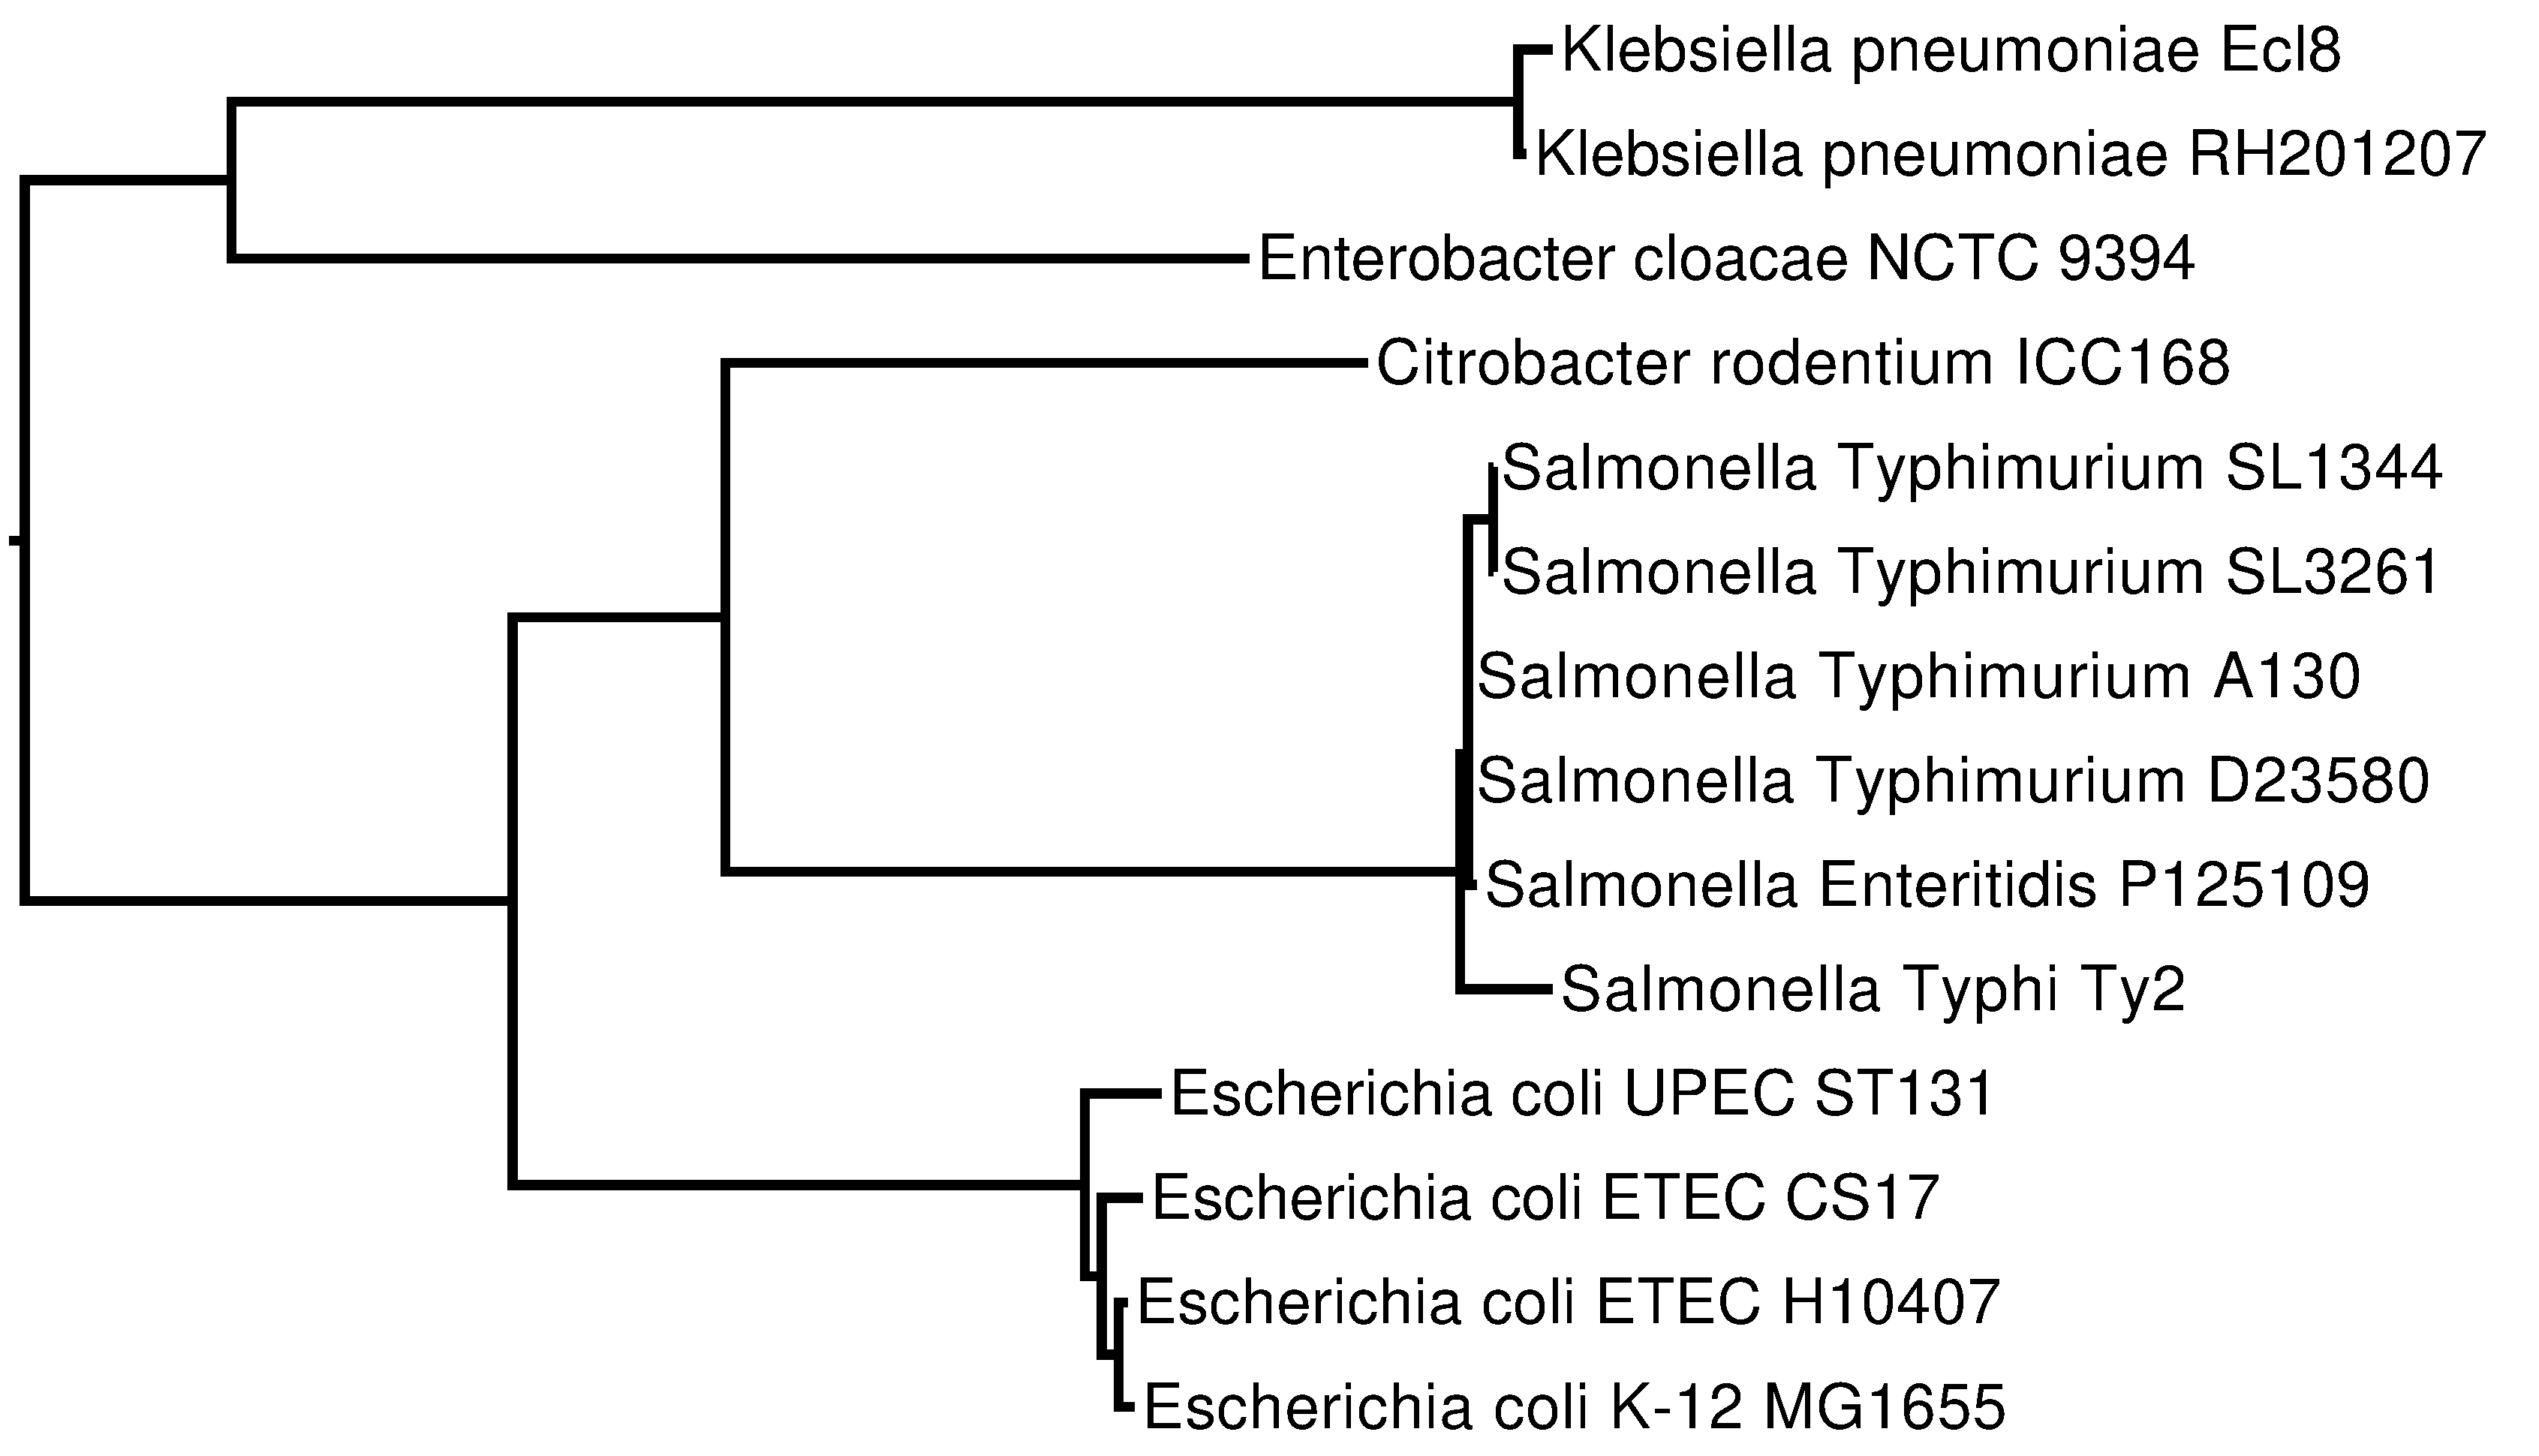
\includegraphics[scale=0.3]{phylosift-aa-raxmlbootstrap.pdf}
\caption{The species tree containing the 13 strains under study and Escherichia \textit{coli} K-12 MG1655 studied in Keio collection \cite{baba_construction_2006}. We have generated the tree by running RAxML \cite{stamatakis_raxml_2014} on Phylosift \cite{darling_phylosift:_2014} amino acid markers.}
\label{fig:species-tree}
\end{figure}

\begin{figure*}
\centering
\begin{tabular}{c c c}
\includegraphics[page=2, scale=0.25]{biases.pdf}&
\includegraphics[page=5, scale=0.25]{biases.pdf}&
\includegraphics[page=8, scale=0.25]{biases.pdf}\\
\includegraphics[page=11, scale=0.25]{biases.pdf}&
\includegraphics[page=14, scale=0.25]{biases.pdf}&
\includegraphics[page=17, scale=0.25]{biases.pdf}\\
\includegraphics[page=20, scale=0.25]{biases.pdf}&
\includegraphics[page=23, scale=0.25]{biases.pdf}&
\includegraphics[page=26, scale=0.25]{biases.pdf}\\
\includegraphics[page=29, scale=0.25]{biases.pdf}&
\includegraphics[page=32, scale=0.25]{biases.pdf}&
\includegraphics[page=35, scale=0.25]{biases.pdf}\\
&\includegraphics[page=38, scale=0.25]{biases.pdf}&\\
\end{tabular}
\caption{The plots show the position of the genes within the genome (normalised by the lengths of the genomes) versus the insertion indices of the genes}
\label{fig:distance-bias}
\end{figure*}

\begin{figure*}
\begin{tabular}{c c}
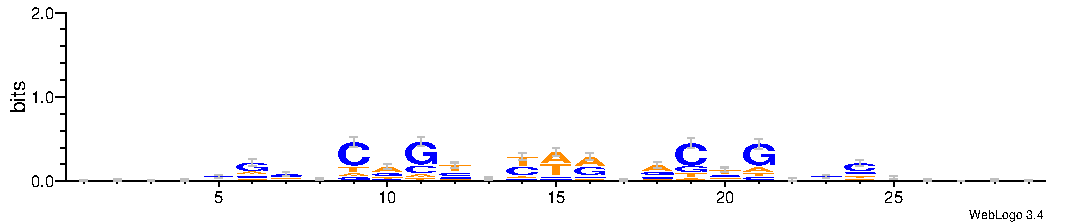
\includegraphics[scale=0.6]{100logo-bits.pdf}&
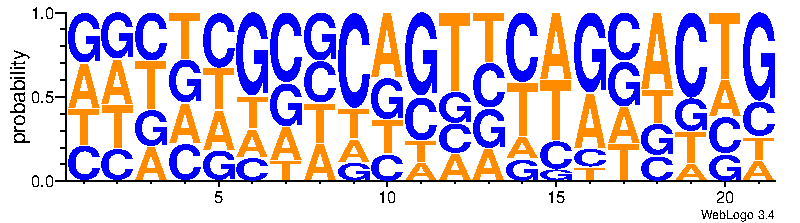
\includegraphics[scale=0.6]{100logo-prob.pdf}
\end{tabular}
\caption{We have generated the logos from 10 nucleotides flanking the 100 top most frequent insertion sites.}
\label{fig:logos}
\end{figure*}

\begin{figure*}
\centering
\begin{tabular}{c c c}
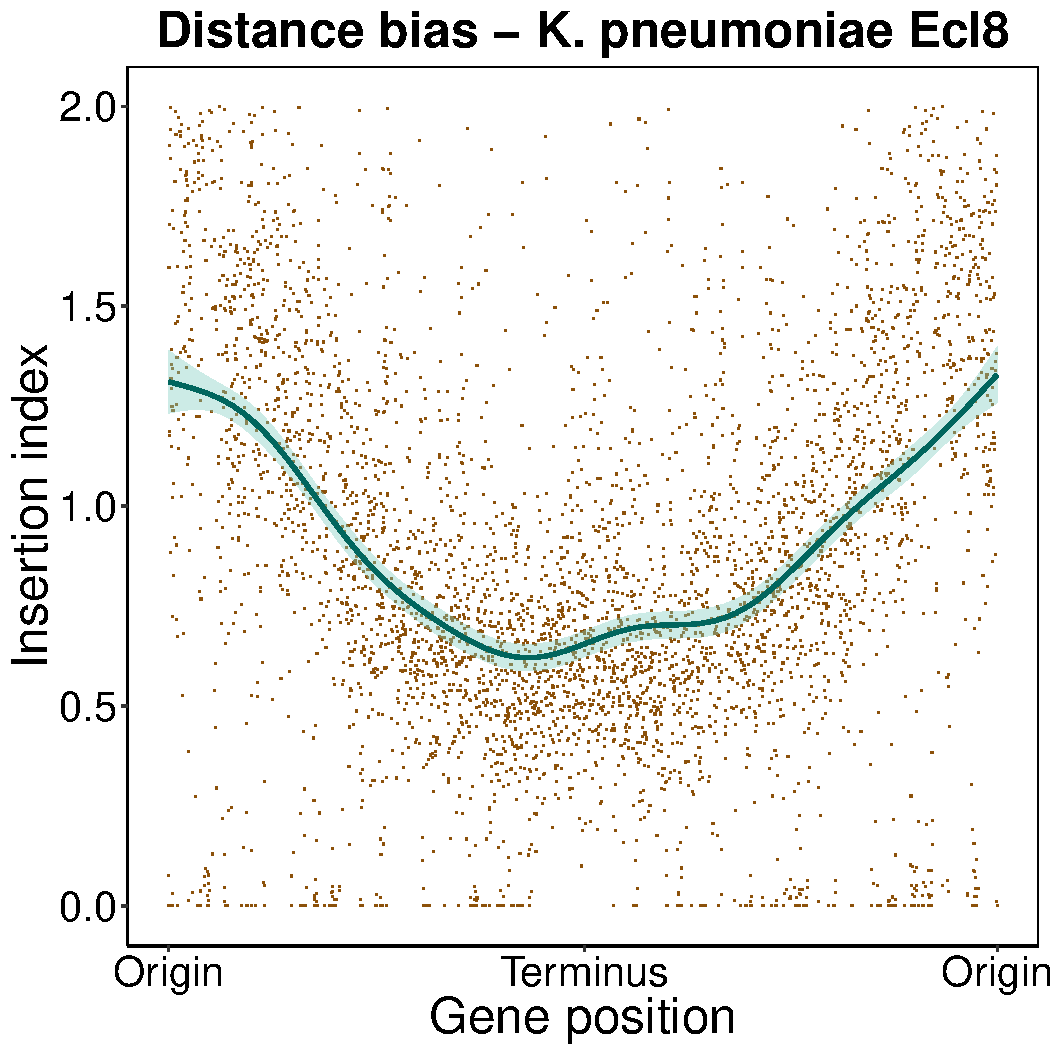
\includegraphics[page=1, scale=0.25]{biases.pdf}&
\includegraphics[page=4, scale=0.25]{biases.pdf}&
\includegraphics[page=7, scale=0.25]{biases.pdf}\\
\includegraphics[page=10, scale=0.25]{biases.pdf}&
\includegraphics[page=13, scale=0.25]{biases.pdf}&
\includegraphics[page=16, scale=0.25]{biases.pdf}\\
\includegraphics[page=19, scale=0.25]{biases.pdf}&
\includegraphics[page=22, scale=0.25]{biases.pdf}&
\includegraphics[page=25, scale=0.25]{biases.pdf}\\
\includegraphics[page=28, scale=0.25]{biases.pdf}&
\includegraphics[page=31, scale=0.25]{biases.pdf}&
\includegraphics[page=34, scale=0.25]{biases.pdf}\\
&\includegraphics[page=37, scale=0.25]{biases.pdf}&\\
\end{tabular}
\caption{The plots show the G-C contents of the genes (normalised by the lengths of the genes) against their insertion indices}
\label{fig:GC-bias}
\end{figure*}

\begin{figure*}
\begin{tabular}{c c}
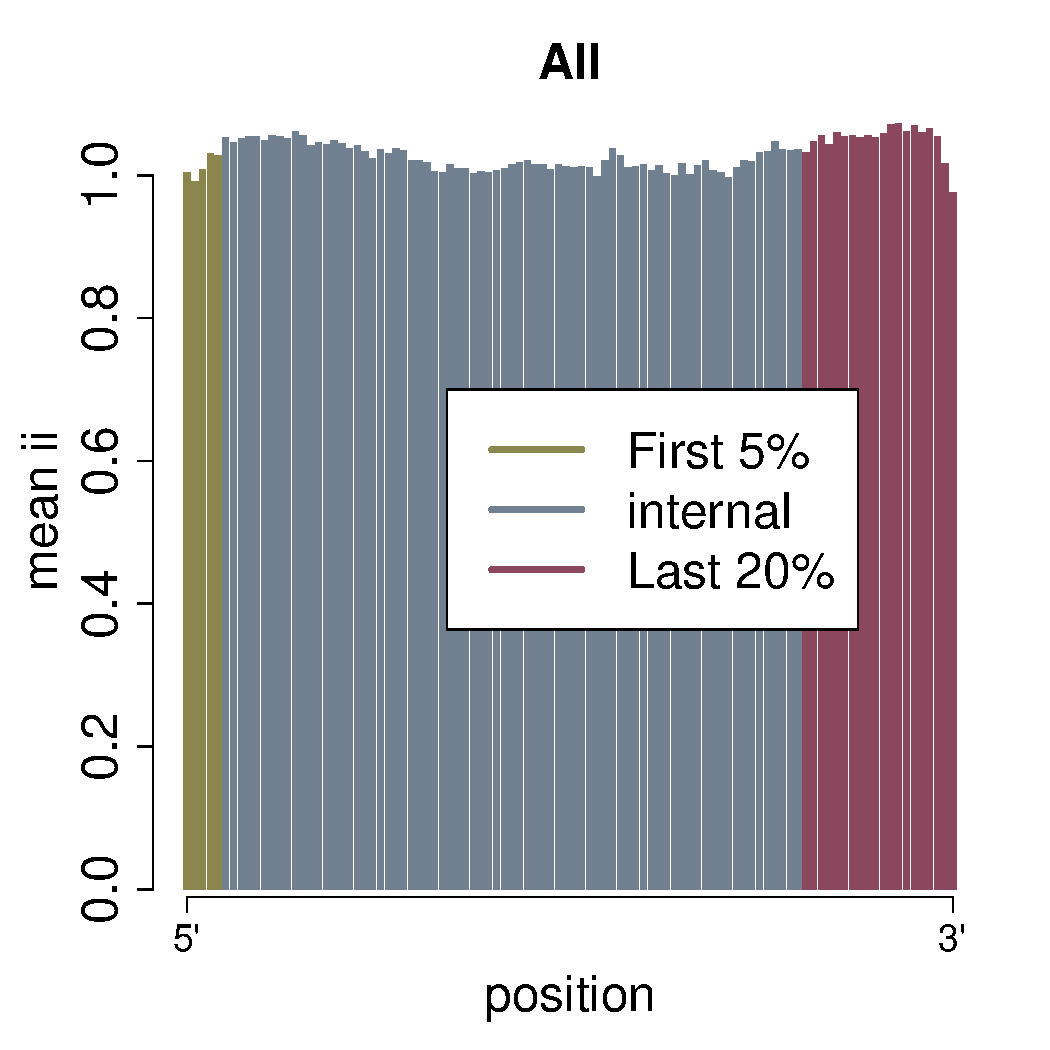
\includegraphics[scale=0.5, page=1]{insertion-position-bias.pdf}&
\includegraphics[scale=0.5, page=2]{insertion-position-bias.pdf}\\
\includegraphics[scale=0.5, page=3]{insertion-position-bias.pdf}&
\includegraphics[scale=0.5, page=4]{insertion-position-bias.pdf}
\end{tabular}
\caption{We have divided our genes into 3 segments: 5\% of
the genes on the 5’ end, 20\% of the genes on the 3’ end, and the rest in the middle.}
\label{fig:insertion-position-bias}
\end{figure*}

\begin{figure}
\centering
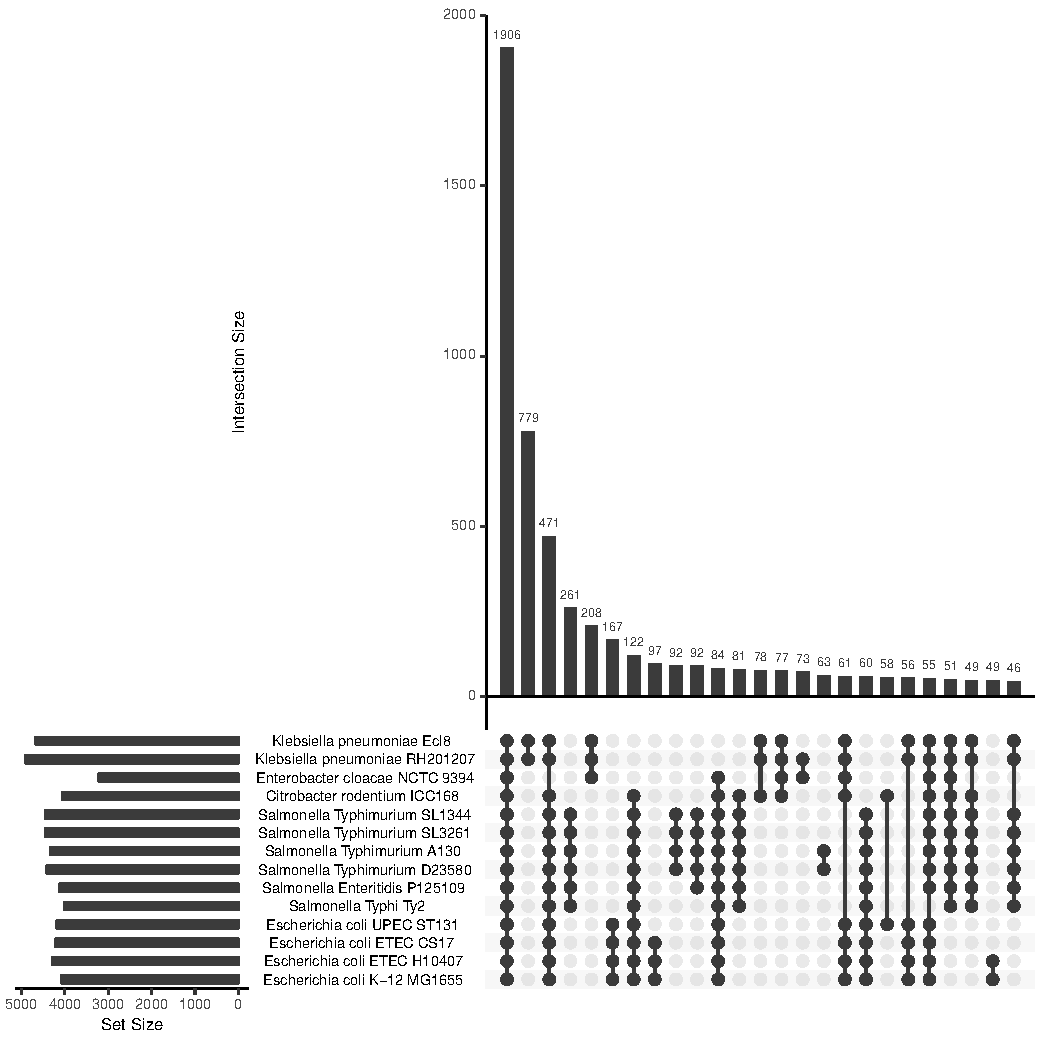
\includegraphics[scale=0.65, page=1]{upsetr.pdf}\\
\includegraphics[scale=0.65, page=2]{upsetr.pdf}
\caption{The first figure shows the number of core genes between each group of species and the second figure shows the number of core essential genes.}
\label{fig:upsetr}
\end{figure}

%----------------------------------------------------------------------------------------

\end{document}